\section{Software In the Loop Testing}

In order to simulate an aircraft tracking the optimized path, a software in the loop (SITL) simulation will be performed. For this the applications Dune, ArduPilot and Neptus will be used. A short explanation of each of these will be given in the following sections.

%\begin{figure}[h]
%	\centering
%    \makebox[\textwidth][c]{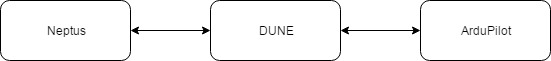
\includegraphics[width=\textwidth, keepaspectratio=true]{sitl_overview.jpg}}
%	\caption{An overview of what information the modules share.}
%	\label{fig:sitl_overview}
%\end{figure}

\subsection{DUNE}

DUNE Unified Navigation Environment is a part of the LSTS toolchain (Laboratório de Sistemas e Tecnologia Subaquática) which aims to provide a control architecture that will ease the control of unmanned air, ground surface and underwater vehicles \cite{DUNE}. DUNE is the software intended to run on board the unmanned vehicles, and provides an interface towards sensor drivers, and navigation and control functionality. In this thesis DUNE will be used to turn the flight path into waypoints that can be sent to the autopilot.

The functionality needed to track the path is made as a \textit{task} using the application programming interface (API) provided by DUNE. The task receives information about the UAV states from the vehicle, and uses this information to provide meaningful input to the autopilot depending on the stage of the operation. When generating waypoints from the path the task uses the principle of \textit{Line-of-Sight} (LOS) guidance to find waypoints a given distance away from the vehicle.


\subsection{ArduPilot}

ArduPilot is an open-source autopilot, which supports several types of vehicles \cite{ARDUPILOT}. It provides functionality for SITL simulation by interfacing the flight dynamics model provided by JSBSim \cite{JSBSim}. ArduPilot communicates with DUNE to receive control commands and send information about the UAV states.


\subsection{Neptus}

Neptus is also a part of the LSTS toolchain, and is used to execute the simulations, and generate logs after they are finished \cite{NEPTUS}. It provides a map interface to observe the simulations in real-time, and also displays information about the aircraft. It communicates with DUNE throught using IMC messages based on a control message set defined by the LSTS toolchain.